\documentclass[10 pt,usenames,dvipsnames, oneside]{article}
\usepackage{../../../modelo-ensino-medio}



\begin{document}

\begin{center}
  \begin{minipage}[l]{3cm}

\includegraphics[width=2cm]{logo}    
\end{minipage}\hfill
\begin{minipage}[r]{.8\textwidth}
 {\Large \scshape Atividade: Bolinha na roda da bibicleta}  
\end{minipage}
\end{center}
\vspace{.2cm}

\ifdefined\prof
%Habilidades da BNCC
% \begin{objetivos}
% \item 
% \end{objetivos}

%Caixa do Para o Professor
\begin{goals}
%Objetivos específicos
\begin{enumerate}
\item Familiarizar o estudante com os arcos e ângulos mais comumente encontrados no estudo de trigonometria na circunferência.
\item Introduzir a ideia do seno e do cosseno como “distâncias orientadas”{} de pontos no círculo aos eixos coordenados.
\end{enumerate}

\tcblower

%Orientações e sugestões
Professor, procure ajudar os alunos a associar os valores encontrados nessa atividade às coordenadas do ponto sobre o qual está a extremidade do arco em estudo, ou a bolinha amarela.
\end{goals}

\bigskip
\begin{center}
{\large \scshape Atividade}
\end{center}
\fi

\textit{(Adaptado de Costa (2017))}

Mateus gosta muito de andar de bicicleta e para enfeitar suas rodas, costuma prender bolinhas de tênis nelas (vide figura). Suponha que ele virou a bicicleta de cabeça para baixo, prendeu a bolinha e começou a girar a roda. Na figura a seguir, a imagem à direita ilustra uma representação da roda destacando eixos coordenados e ângulos em graus.

\begin{figure}[H]
\centering

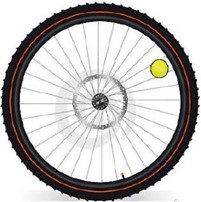
\includegraphics[width=.24\linewidth]{trigonometricas57}
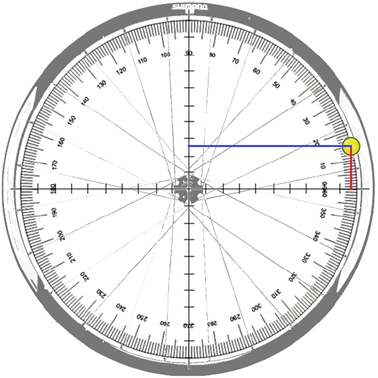
\includegraphics[width=.39\linewidth]{trigonometricas58}
\end{figure}


A roda da direita tem um transferidor de volta inteira sobreposto a sua imagem, de forma que é possível verificar a medida do ângulo entre o eixo horizontal e o raio da roda que passa pela bolinha.

Considere que $r$ é o raio da roda, $c$ é o comprimento do segmento horizontal azul (distância da bolinha amarela ao eixo $y$) e $s$ é o comprimento do segmento vertical vermelho (distância da bolinha amarela ao eixo $x$). A razão $\frac{c}{r}$ indica a distância horizontal relativa entre a bolinha amarela e o eixo $y$, assim como a razão $\frac{s}{r}$ indica a distância vertical relativa entre a bolinha amarela e o eixo $x$. Por exemplo, se a roda tem raio de $30$ cm e a bolinha estiver localizada a $27$ cm do eixo vertical, então $\frac{c}{r}$ é $\frac{27}{30}$, ou seja, $\frac{9}{10}$. Dessa forma, para quaisquer outras rodas de bicicleta com outros raios, quando o ângulo entre o eixo horizontal e o raio que passa pela bolinha amarela for o mesmo em que é nessa situação, estamos aptos a determinar essa distância, fundamentados na semelhança de triângulos: em uma roda com $20$ cm de raio, essa distância seria $\frac{9}{10}$ de $20$, ou seja, $18$ cm. Da mesma forma se dá para a distância relativa vertical. Observe ainda que essa “distância relativa”{} pode ser ainda negativa ou positiva, de acordo com a orientação dos eixos coordenados.


\begin{wrapfigure}[8]{l}{.3\linewidth}
\vspace{-1em}
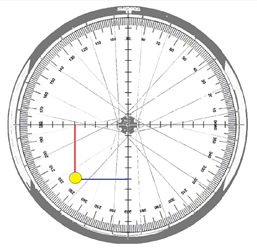
\includegraphics[width=\linewidth]{trigonometricas59}
\end{wrapfigure}

Por exemplo, na figura ao lado, tanto $c$ quanto $s$ valem $5$, mas estão no sentido negativo de seus respectivos eixos, portanto, ao calcularmos as distâncias relativas teremos $\frac{c}{r}=\frac{s}{r}=\frac{-5}{10}=\frac{-1}{2}$.  

Nas tabelas a seguir, temos algumas possíveis posições para a bolinha e os ângulos associados a elas, medidos em graus. Para completar essa tabela, você precisará informar, a cada ângulo dado:

\begin{itemize}
\item A medida do arco, em radianos, associado ao ângulo dado;
\item A razão $\frac{c}{r}$ e o seu sinal, de acordo com a orientação no eixo $x$;
\item A razão $\frac{s}{r}$ e o seu sinal, de acordo com a orientação no eixo $y$.
\end{itemize}

Vamos lá?



\begin{enumerate}
\item \adjustbox{valign=t}
{
\begin{tabular}{|>$e{.15\linewidth}<$|*{6}{>$e{.1\linewidth}<$|}}
\hline
$\tcolor{Ângulo (grau)}$ & \tmat{15^{\circ}} & \tmat{30^{\circ}} & \tmat{45^{\circ}} & \tmat{60^{\circ}} & \tmat{75^{\circ}} & \tmat{90^{\circ}} \tabularnewline
\hline
$\tcolor{Arco (radiano)}$ & \dfrac{\pi}{12} & & & & & \tabularnewline
\hline
\tmat{\dfrac{c}{r}} & 0{,}96 & & & & & \tabularnewline
\hline
\tmat{\dfrac{s}{r}} & 0{,}26 & & & & & \tabularnewline
\hline
\end{tabular}
}


\item \adjustbox{valign=t}
{
\begin{tabular}{|>$e{.15\linewidth}<$|*{6}{>$e{.1\linewidth}<$|}}
\hline
$\tcolor{Ângulo (grau)}$ & \tmat{105^{\circ}} & \tmat{120^{\circ}} & \tmat{135^{\circ}} & \tmat{150^{\circ}} & \tmat{165^{\circ}} & \tmat{180^{\circ}} \tabularnewline
\hline
$\tcolor{Arco (radiano)}$ & & & & & & \tabularnewline
\hline
\tmat{\dfrac{c}{r}} &  & & & & & \tabularnewline
\hline
\tmat{\dfrac{s}{r}} &  & & & & & \tabularnewline
\hline
\end{tabular}
}


\item \adjustbox{valign=t}
{
\begin{tabular}{|>$e{.15\linewidth}<$|*{6}{>$e{.1\linewidth}<$|}}
\hline
$\tcolor{Ângulo (grau)}$ & \tmat{195^{\circ}} & \tmat{210^{\circ}} & \tmat{225^{\circ}} & \tmat{240^{\circ}} & \tmat{255^{\circ}} & \tmat{270^{\circ}} \tabularnewline
\hline
$\tcolor{Arco (radiano)}$ & & & & & & \tabularnewline
\hline
\tmat{\dfrac{c}{r}} &  & & & & & \tabularnewline
\hline
\tmat{\dfrac{s}{r}} &  & & & & & \tabularnewline
\hline
\end{tabular}
}


\item \adjustbox{valign=t}
{
\begin{tabular}{|>$e{.15\linewidth}<$|*{6}{>$e{.1\linewidth}<$|}}
\hline
$\tcolor{Ângulo (grau)}$ & \tmat{285^{\circ}} & \tmat{300^{\circ}} & \tmat{315^{\circ}} & \tmat{330^{\circ}} & \tmat{345^{\circ}} & \tmat{360^{\circ}} \tabularnewline
\hline
$\tcolor{Arco (radiano)}$ & & & & & & 2\pi \tabularnewline
\hline
\tmat{\dfrac{c}{r}} &  & & & & & \tabularnewline
\hline
\tmat{\dfrac{s}{r}} &  & & & & & \tabularnewline
\hline
\end{tabular}
}
\end{enumerate}

\ifdefined\prof
\begin{solucao}

\begin{enumerate}[left=0pt, wide]
\item \phantom{a}

\begin{tabular}{|>$e{.15\linewidth}<$|*{6}{>{$\displaystyle}e{.1\linewidth}<$|}}
\hline
$\tcolor{Ângulo (grau)}$ & \tmat{15^{\circ}} & \tmat{30^{\circ}} & \tmat{45^{\circ}} & \tmat{60^{\circ}} & \tmat{75^{\circ}} & \tmat{90^{\circ}} \tabularnewline
\hline
$\tcolor{Arco (radiano)}$ & \frac{\pi}{12} & \frac{\pi}{6} & \frac{\pi}{4} & \frac{\pi}{3} & \frac{5\pi}{12} & \frac{\pi}{2} \tabularnewline
\hline
\tmat{\dfrac{c}{r}} & 0{,}96 & 0{,}86 & 0{,}7 & 0{,}5 & 0{,}26 & 0 \tabularnewline
\hline
\tmat{\dfrac{s}{r}} & 0{,}26 & 0{,}5 & 0{,}7 & 0{,}86 & 0{,}96 & 1 \tabularnewline
\hline
\end{tabular}



\item \phantom{a}

\begin{tabular}{|>$e{.15\linewidth}<$|*{6}{>{$\displaystyle}e{.1\linewidth}<$|}}
\hline
$\tcolor{Ângulo (grau)}$ & \tmat{105^{\circ}} & \tmat{120^{\circ}} & \tmat{135^{\circ}} & \tmat{150^{\circ}} & \tmat{165^{\circ}} & \tmat{180^{\circ}} \tabularnewline
\hline
$\tcolor{Arco (radiano)}$ & \frac{7\pi}{12} & \frac{2\pi}{3} & \frac{3\pi}{6} & \frac{5\pi}{6} & \frac{11\pi}{12} & \pi \tabularnewline
\hline
\tmat{\dfrac{c}{r}} & -0{,}25 & -0{,}5 & -0{,}7 & -0{,}86 & -0{,}96 & -1 \tabularnewline
\hline
\tmat{\dfrac{s}{r}} & 0{,}96 & 0{,}86 & 0{,}7 & 0{,}5 & 0{,}26 & 0 \tabularnewline
\hline
\end{tabular}


\item \phantom{a}

\begin{tabular}{|>$e{.15\linewidth}<$|*{6}{>{$\displaystyle}e{.1\linewidth}<$|}}
\hline
$\tcolor{Ângulo (grau)}$ & \tmat{195^{\circ}} & \tmat{210^{\circ}} & \tmat{225^{\circ}} & \tmat{240^{\circ}} & \tmat{255^{\circ}} & \tmat{270^{\circ}} \tabularnewline
\hline
$\tcolor{Arco (radiano)}$ &\frac{13\pi}{12}  & \frac{7\pi}{6} & \frac{5\pi}{4} & \frac{4\pi}{3} & \frac{17\pi}{12} & 2\pi \tabularnewline
\hline
\tmat{\dfrac{c}{r}} & -0{,}96 & -0{,}86 & -0{,}7 & -0{,}5 & -0{,}26 & 0 \tabularnewline
\hline
\tmat{\dfrac{s}{r}} & -0{,}26 & -0{,}5 & -0{,}7 & -0{,}86 & -0{,}96 & -1 \tabularnewline
\hline
\end{tabular}



\item \phantom{a}

\begin{tabular}{|>$e{.15\linewidth}<$|*{6}{>{$\displaystyle}e{.1\linewidth}<$|}}
\hline
$\tcolor{Ângulo (grau)}$ & \tmat{285^{\circ}} & \tmat{300^{\circ}} & \tmat{315^{\circ}} & \tmat{330^{\circ}} & \tmat{345^{\circ}} & \tmat{360^{\circ}} \tabularnewline
\hline
$\tcolor{Arco (radiano)}$ &\frac{19\pi}{12}  & \frac{5\pi}{3} & \frac{7\pi}{4} & \frac{11\pi}{6} & \frac{23\pi}{12} & 2\pi \tabularnewline
\hline
\tmat{\dfrac{s}{r}} & 0{,}26 & 0{,}5 & 0{,}7 & 0{,}86 & 0{,}96 & 1 \tabularnewline
\hline
\tmat{\dfrac{c}{r}} & -0{,}96 & -0{,}86 & -0{,}7 & -0{,}5 & -0{,}26 & 0 \tabularnewline
\hline
\end{tabular}

\end{enumerate}

\end{solucao}
\fi

\end{document}